\section{Frequency mode 17}
\label{FM17}

\subsection{Spectra}
\label{FM17:spectra}

\begin{figure}[ht]
    \centering
    \begin{subfigure}[b]{0.9545\textwidth}
        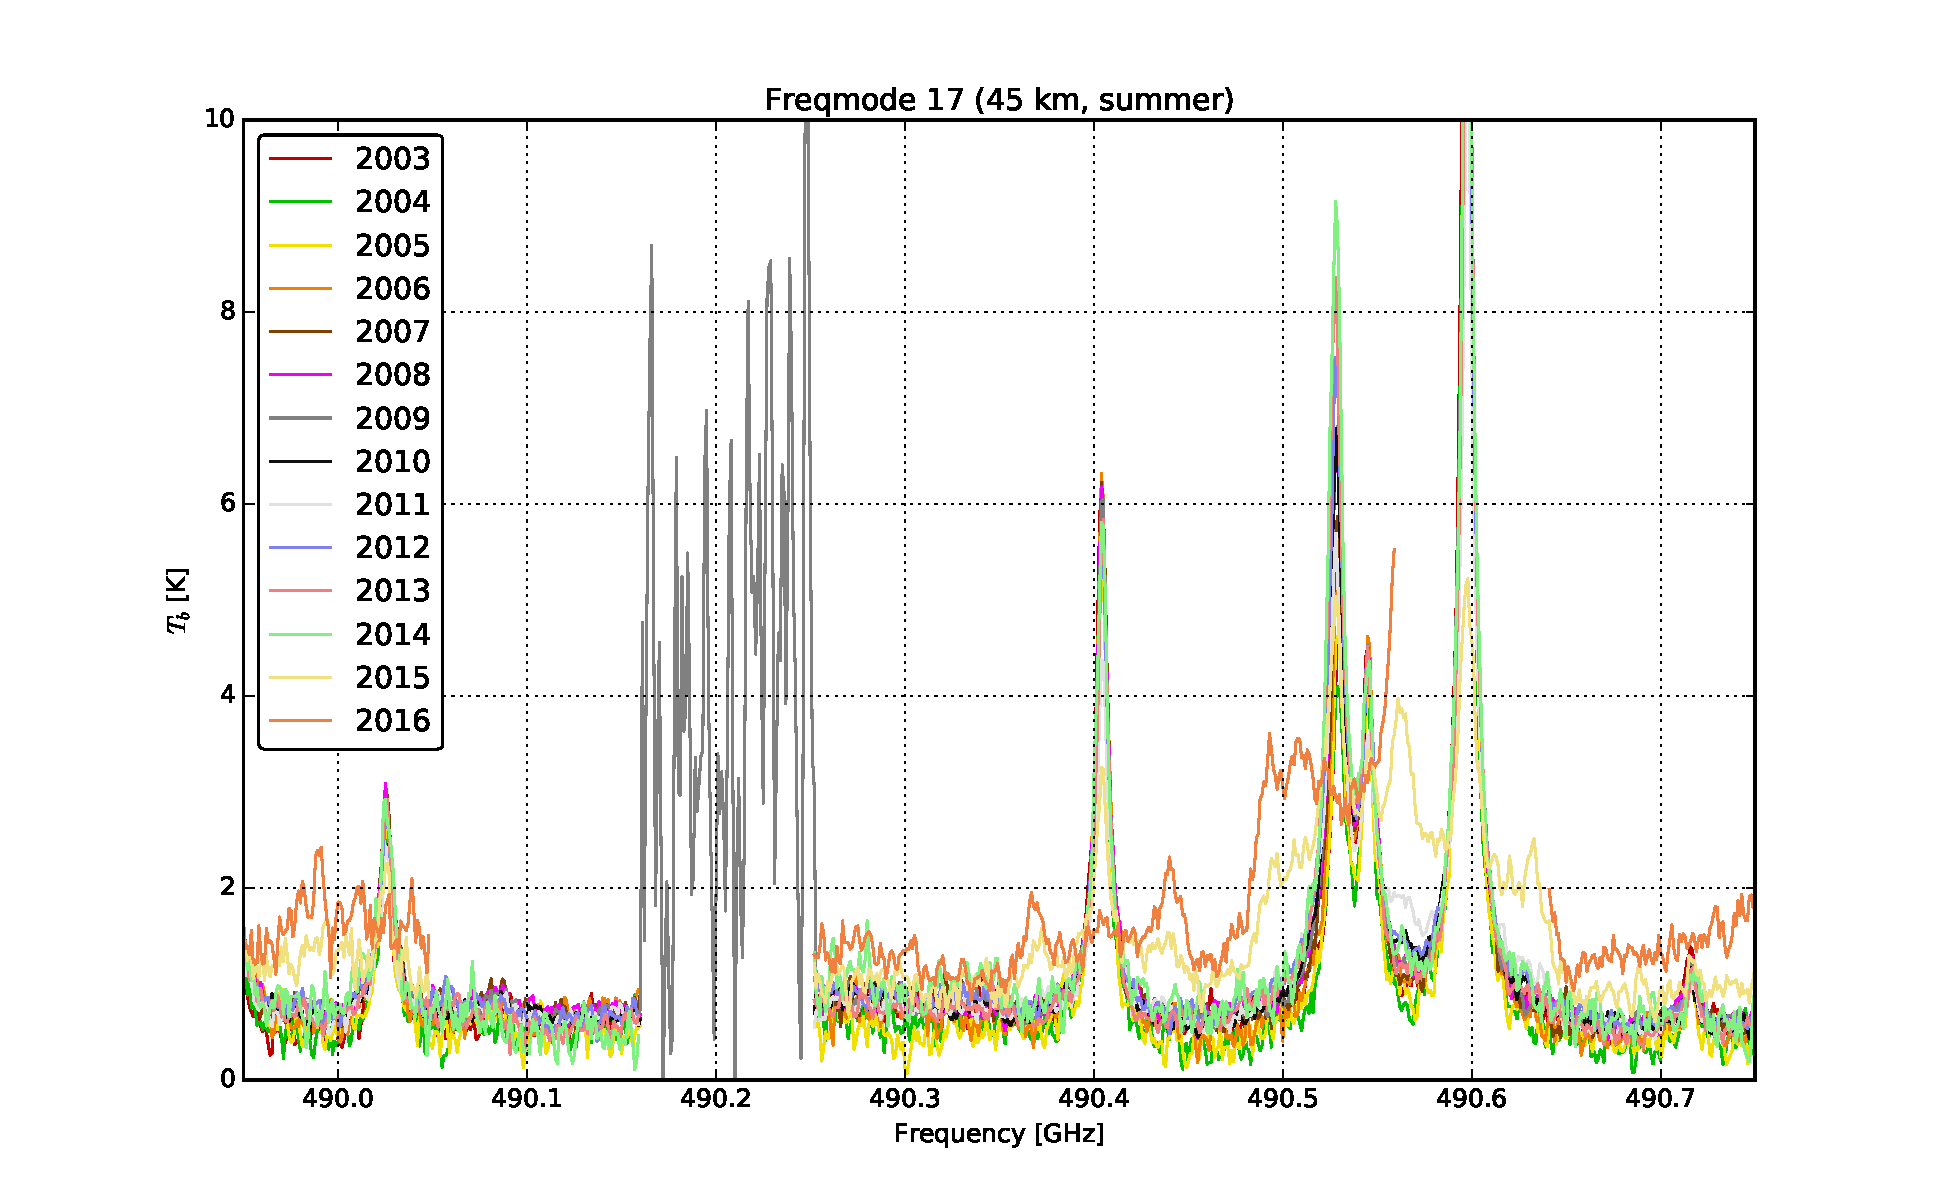
\includegraphics[width=\textwidth]{spectra/fm_17_spectra_summer}
        \caption{summer; 2014--2016 from FM~117}\label{fig:spectra:17:summer}
    \end{subfigure}
    \begin{subfigure}[b]{0.9545\textwidth}
        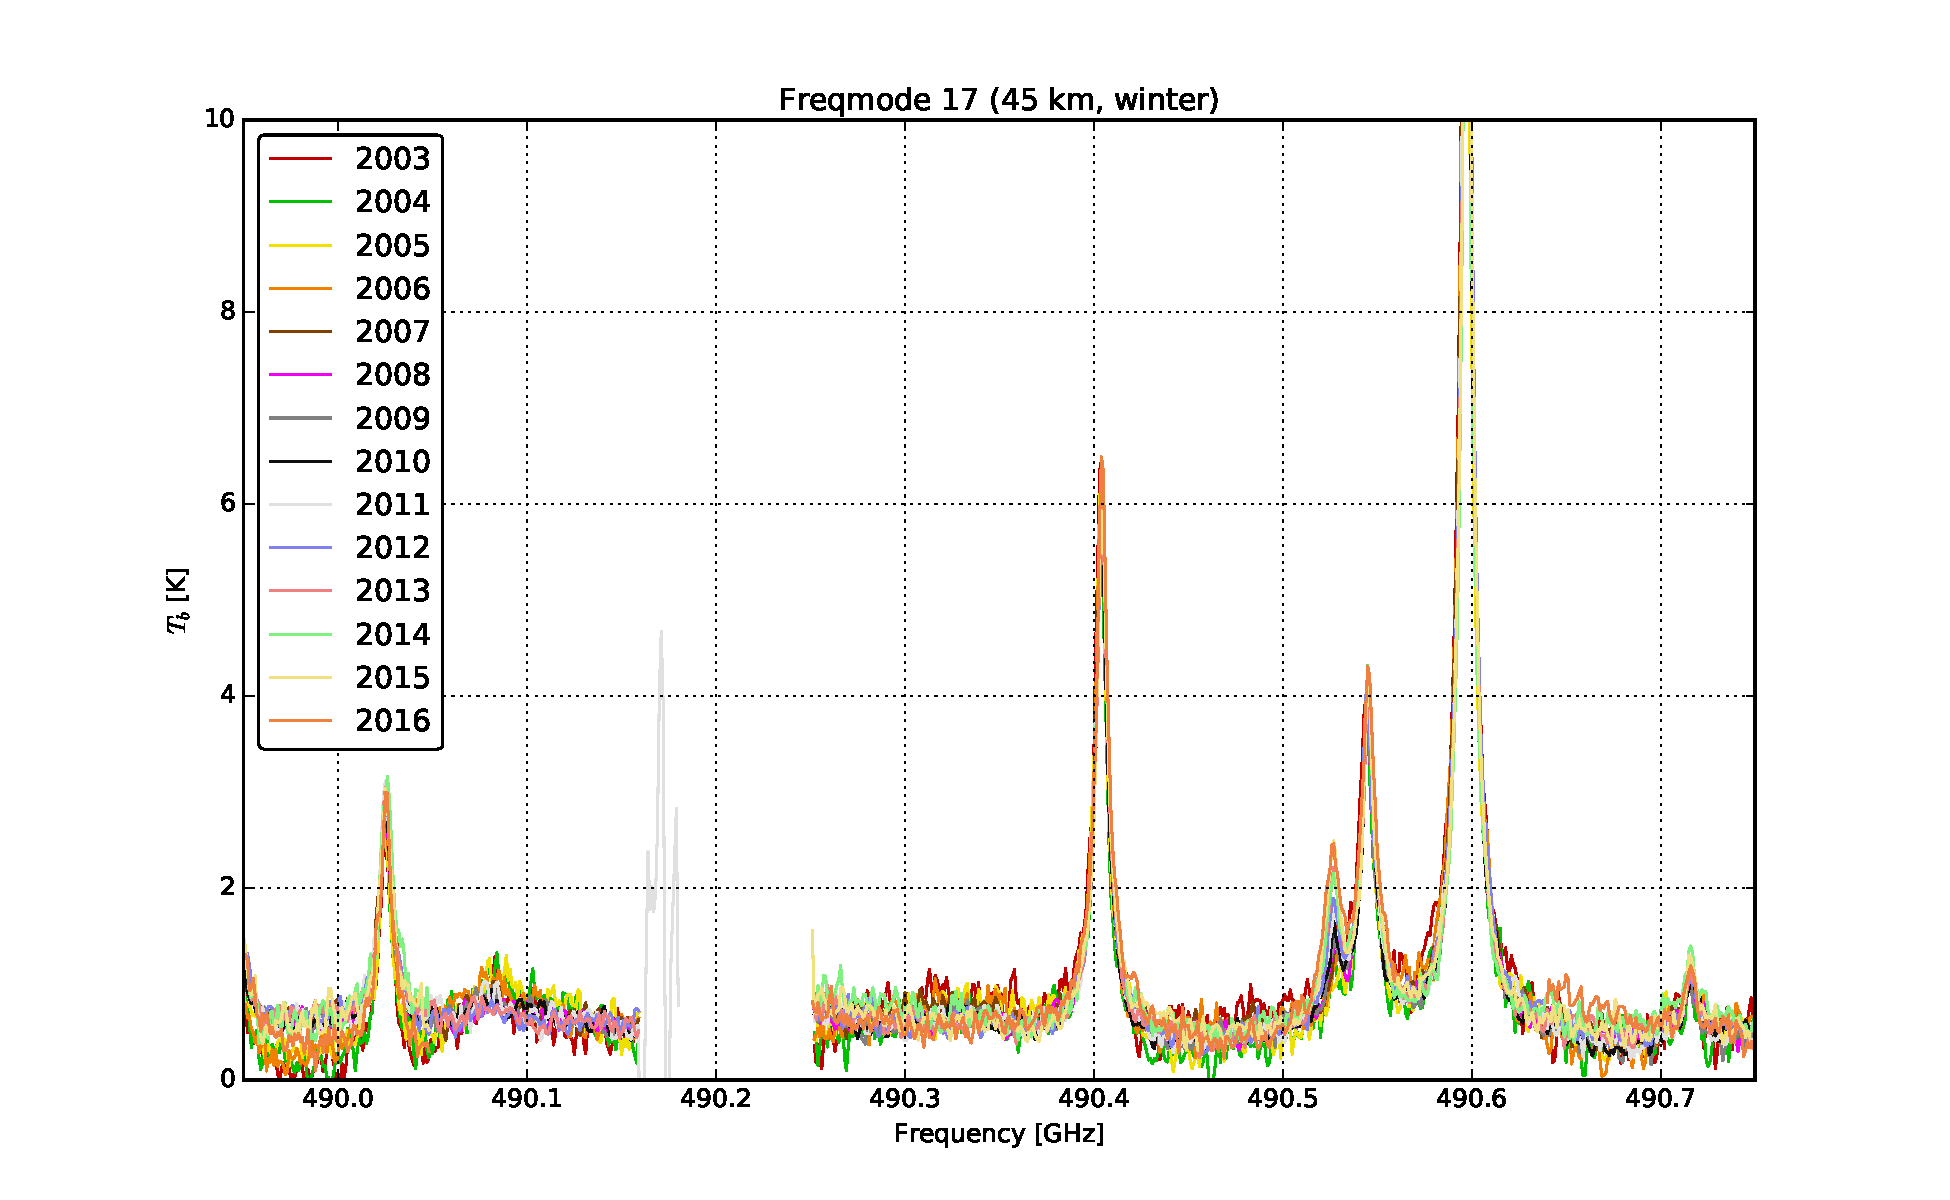
\includegraphics[width=\textwidth]{spectra/fm_17_spectra_winter}
        \caption{winter}\label{fig:spectra:17:winter}
    \end{subfigure}
    \caption{Annual median spectra for FM~17 for altitude interval 40--45~km
        at equatorial latitudes.  The main band peaks are \chem{O^{18}OO}
        at~$\sim490.03\,\mathrm{GHz}$, \chem{OO^{18}O}
        at~$\sim490.40$ and~$490.54\,\mathrm{GHz}$, \chem{HDO}
        at~$\sim490.60\,\mathrm{GHz}$, and \chem{OO^{17}O}
        at~$\sim490.72\,\mathrm{GHz}$.  There is a an \chem{O^3} sideband peak
        from $\sim497.97\,\mathrm{GHz}$ at $\sim490.53\,\mathrm{GHz}$, just
        below the second \chem{OO^{18}O} peak.  The unhealthy sub-bands~7 and~3
        encompass the area bewteen~$\sim490.05$ and~$490.25\,\mathrm{GHz}$.
        }\label{fig:spectra:17}
\end{figure}

\noindent
\TODO{Add FM~17 conclusions}

\subsection{Sideband leakage}
\label{FM17:sbl}

\subsection{Seasonality}
\label{FM17:seasonailty}
